\section{Ristoratore}

\subsection{Header}

\begin{figure}[htbp]
    \centering
	
\includegraphics[width=0.8\textwidth]{PB/manuale-utente/header-ristoratore.png}
    \caption{Barra di Navigazione per il ristoratore}
\end{figure}

La barra di navigazione in alto ti permette di accedere facilmente alle varie 
sezioni della piattaforma:
\begin{itemize}
	\item \texttt{Logo e "Easy Meal"}: cliccando sul logo o sul nome "Easy Meal"
		sei reindirizzato alla Home Page della piattaforma;

	\item \texttt{Esplora}: cliccando su questo riferimento sei reindirizzato
		alla Home Page della piattaforma;

	\item \texttt{Ingredienti}: cliccando su questa voce sei reindirizzato alla
		pagina di gestione degli ingredienti del tuo ristorante;

	\item \texttt{Piatti}: cliccando su questo riferimento sei reindirizzato
		alla pagina di visualizzazione dei piatti del tuo ristorante;

	\item \texttt{Prenotazioni}: cliccando su questo riferimento sei 
		reindirizzato alla pagina di visualizzazione della lista di
		prenotazioni;

	\item \texttt{Notifiche}: cliccando su questo riferimento sei reindirizzato
		alla pagina di visualizzazione della lista di notifiche. Nota che se ci
		sono notifiche non lette, il riferimento sarà seguito da un \textit{badge} che
		indica il numero di notifiche non lette;

	\item \texttt{Logout}: cliccando su questo riferimento effettuerai il \textit{logout}
		dalla piattaforma e sarai reindirizzato alla Home Page della 
		piattaforma.
\end{itemize}

\subsection{Esplora (Home Page)}

Questa pagina è analoga alla Home Page della piattaforma per l'utente generico.

\subsection{Ingredienti}

\begin{figure}[htbp]
    \centering
	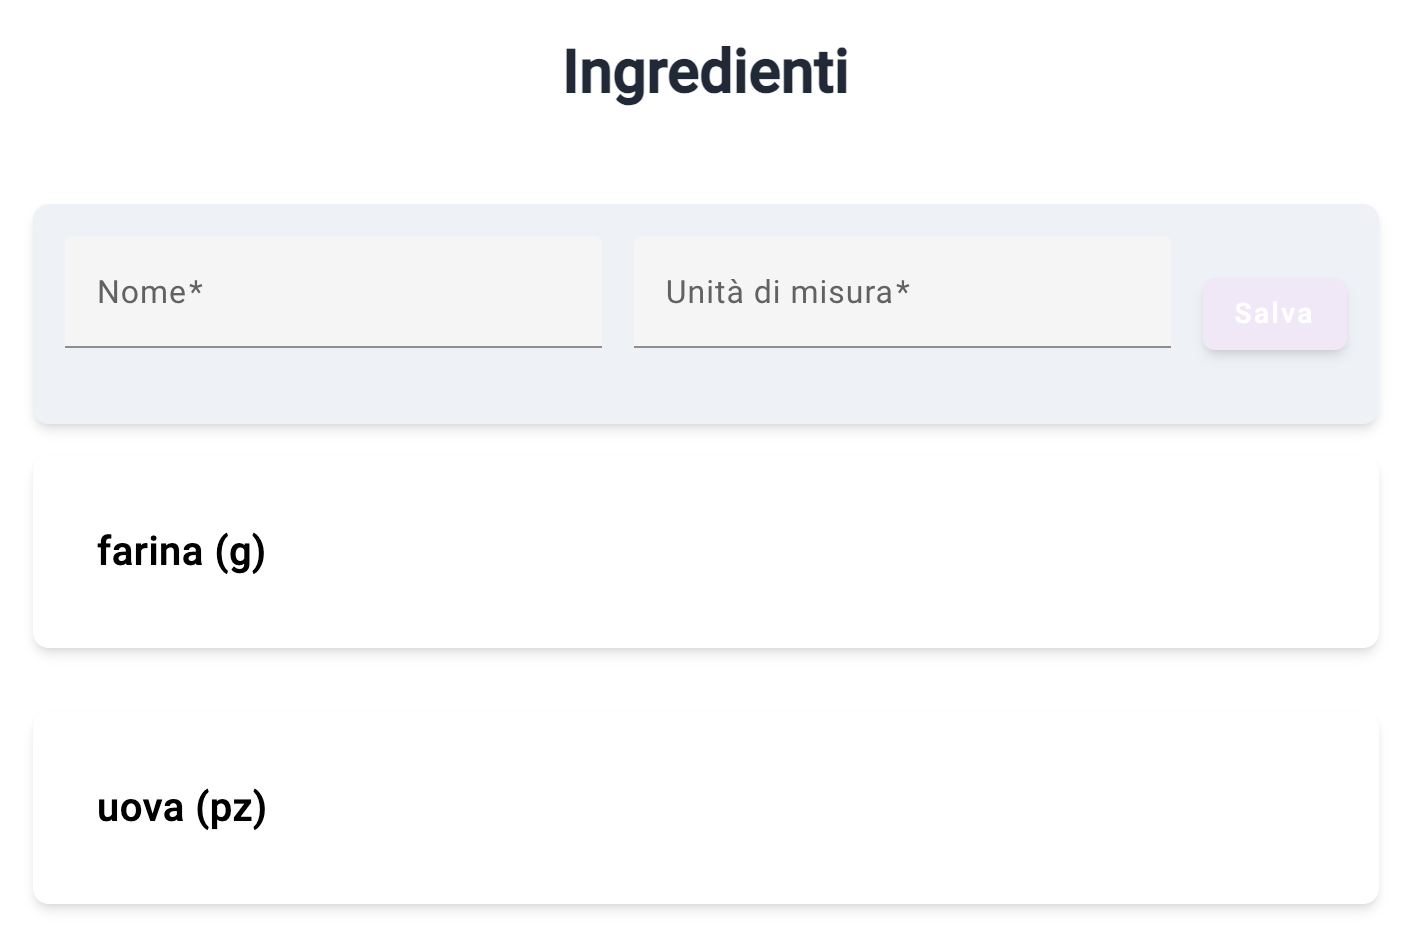
\includegraphics[width=0.8\textwidth]{PB/manuale-utente/ingredienti-ristoratore.png}
    \caption{Pagina di visualizzazione delle prenotazioni per il ristoratore}
\end{figure}

Si accede a questa pagina cliccando su \texttt{Ingredienti} nella barra di
navigazione. Qui puoi visualizzare tutti gli ingredienti presenti nel menu del
tuo ristorante. In cima alla lista degli ingredienti è presente un modulo che
richiede:
\begin{itemize}
	\item Nome: il nome dell'ingrediente;
	\item Unità di misura: l'unità di misura dell'ingrediente. Le opzioni
		disponibili sono: g, ml, p, q.b.
\end{itemize}

Avendo compilato i campi, puoi salvare l'ingrediente cliccando sul pulsante
\texttt{Salva}. Viene visualizzato un messaggio di conferma o di errore
dell'operazione. Sotto il modulo di inserimento sono elencati tutti gli
ingredienti presenti nel menu del ristorante. Puoi modificarli cliccando su di
un ingrediente. Dopo aver cliccato su un ingrediente, esso si trasforma in un
\textit{form} che ti permette di modificare i campi dell'ingrediente. Puoi eliminare
l'ingrediente cliccando sul pulsante \texttt{Elimina} a destra, oppure lo puoi
salvare cliccando sul pulsante \texttt{Salva}.

\subsection{Piatti}

\begin{figure}[htbp]
    \centering
	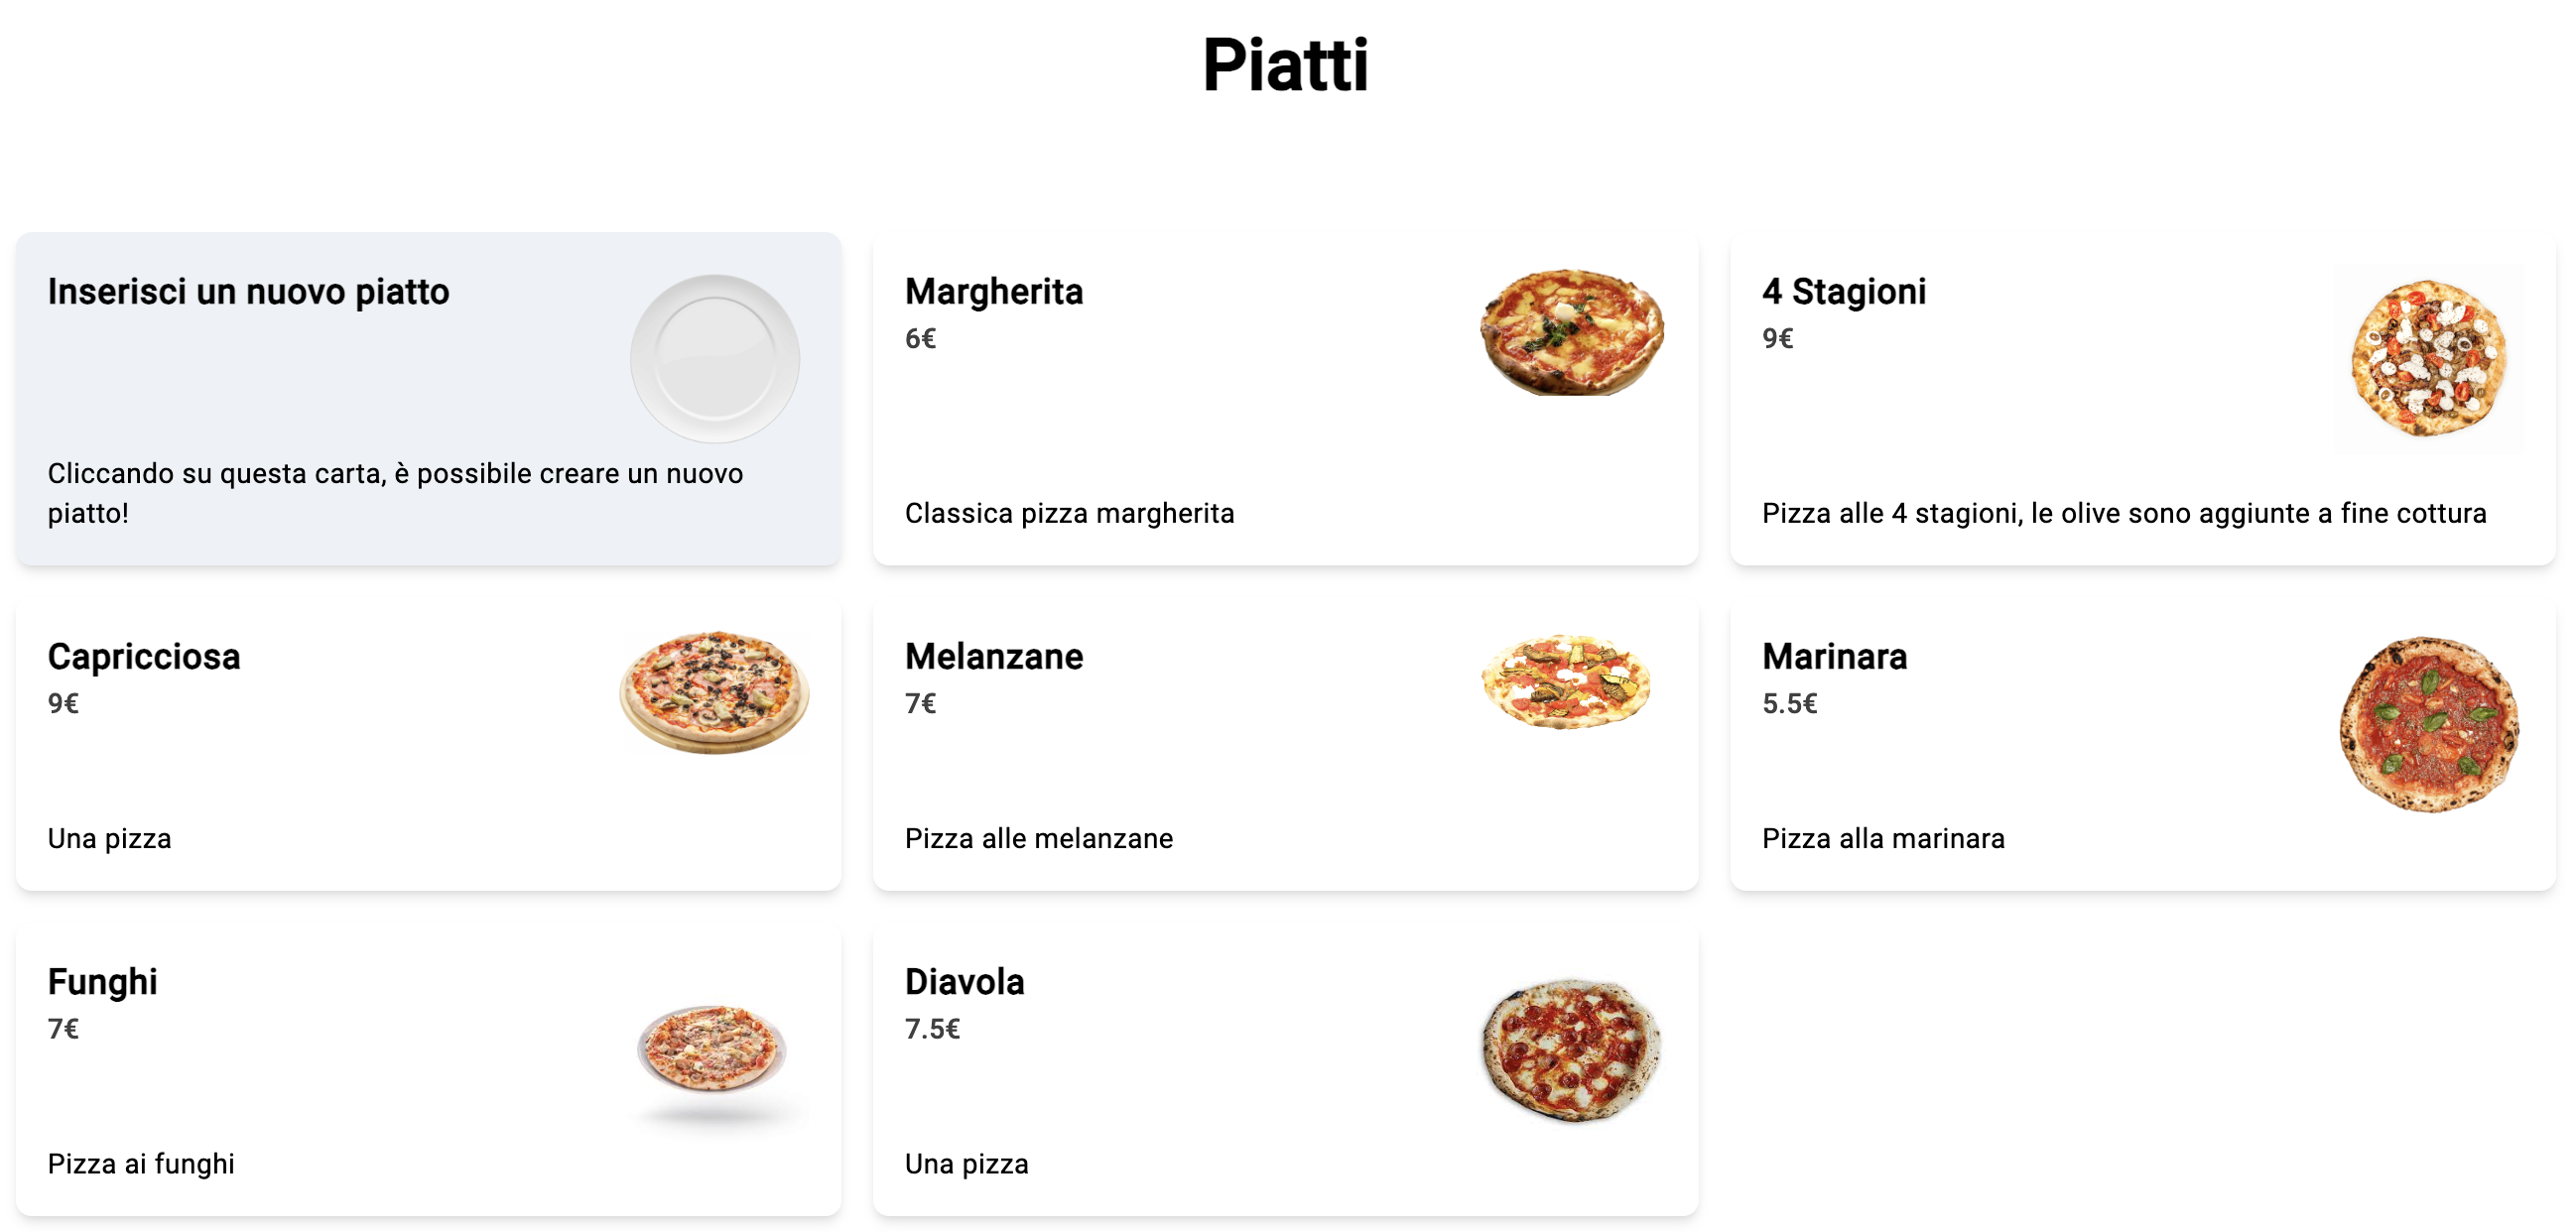
\includegraphics[width=0.8\textwidth]{PB/manuale-utente/piatti-ristoratore.png}
    \caption{Pagina di visualizzazione dei piatti per il ristoratore}
\end{figure}

Si accede a questa pagina cliccando su \texttt{Piatti} nella barra di
navigazione. Qui puoi visualizzare tutti i piatti presenti nel menu del tuo
ristorante. Cliccando su di un piatto si accede alla pagina di dettaglio del
piatto. Cliccando sul primo piatto della lista si accede alla pagina di
inserimento di un nuovo piatto.

\newpage
\subsection{Nuovo piatto}

\begin{figure}[htbp]
    \centering
	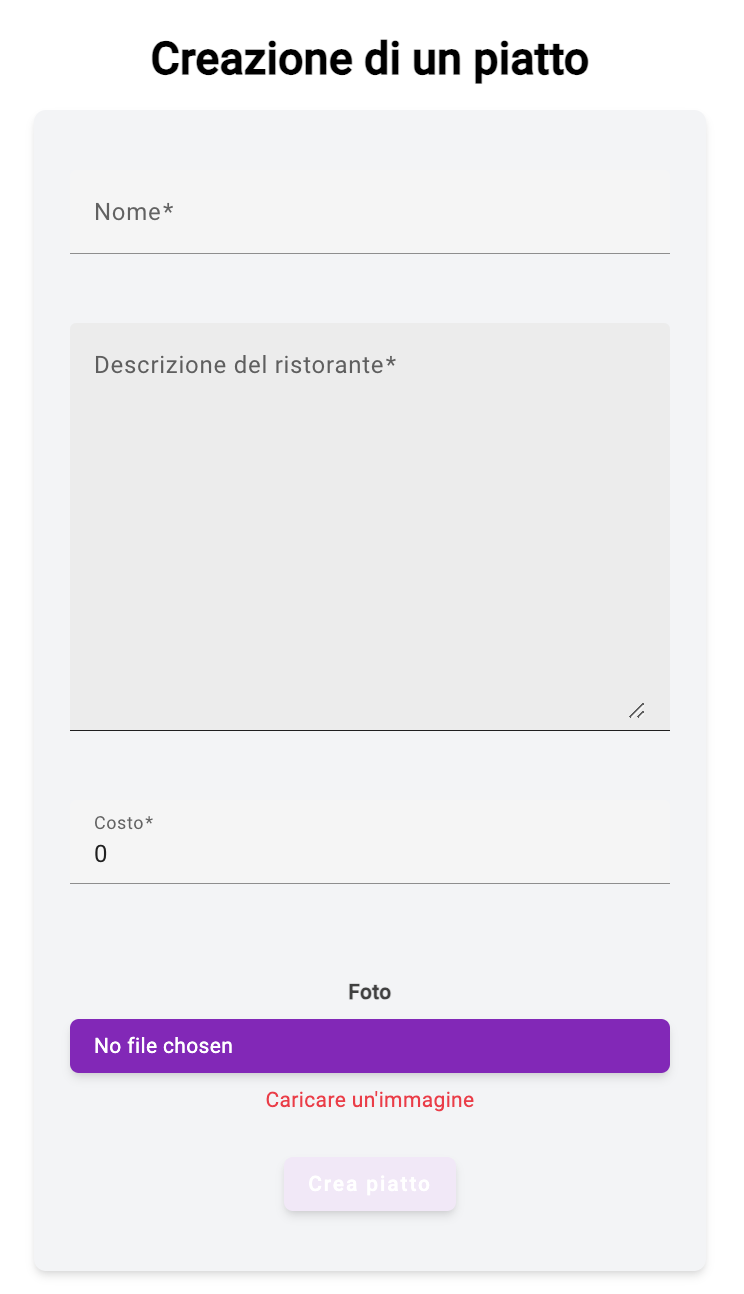
\includegraphics[width=0.6\textwidth]{PB/manuale-utente/nuovo-piatto-ristoratore.png}
    \caption{Pagina di inserimento di un nuovo piatto per il ristoratore}
\end{figure}

Si accede a questa pagina cliccando sul primo piatto della lista dei piatti.
Questa pagina è composta da un \textit{form} che richiede:
\begin{itemize}
	\item Nome;
	\item Descrizione del piatto;
	\item Costo;
	\item Foto.
\end{itemize}

Dopo aver compilato il \textit{form}, puoi salvare il piatto cliccando sul pulsante
\texttt{Crea piatto}. Se l'operazione va a buon fine, vieni reindirizzato alla
pagina di dettaglio del piatto e viene visualizzato un messaggio di conferma di
avvenuta creazione del piatto; altrimenti viene visualizzato un messaggio di
errore.

\subsection{Dettaglio piatto}

\begin{figure}[htbp]
    \centering
	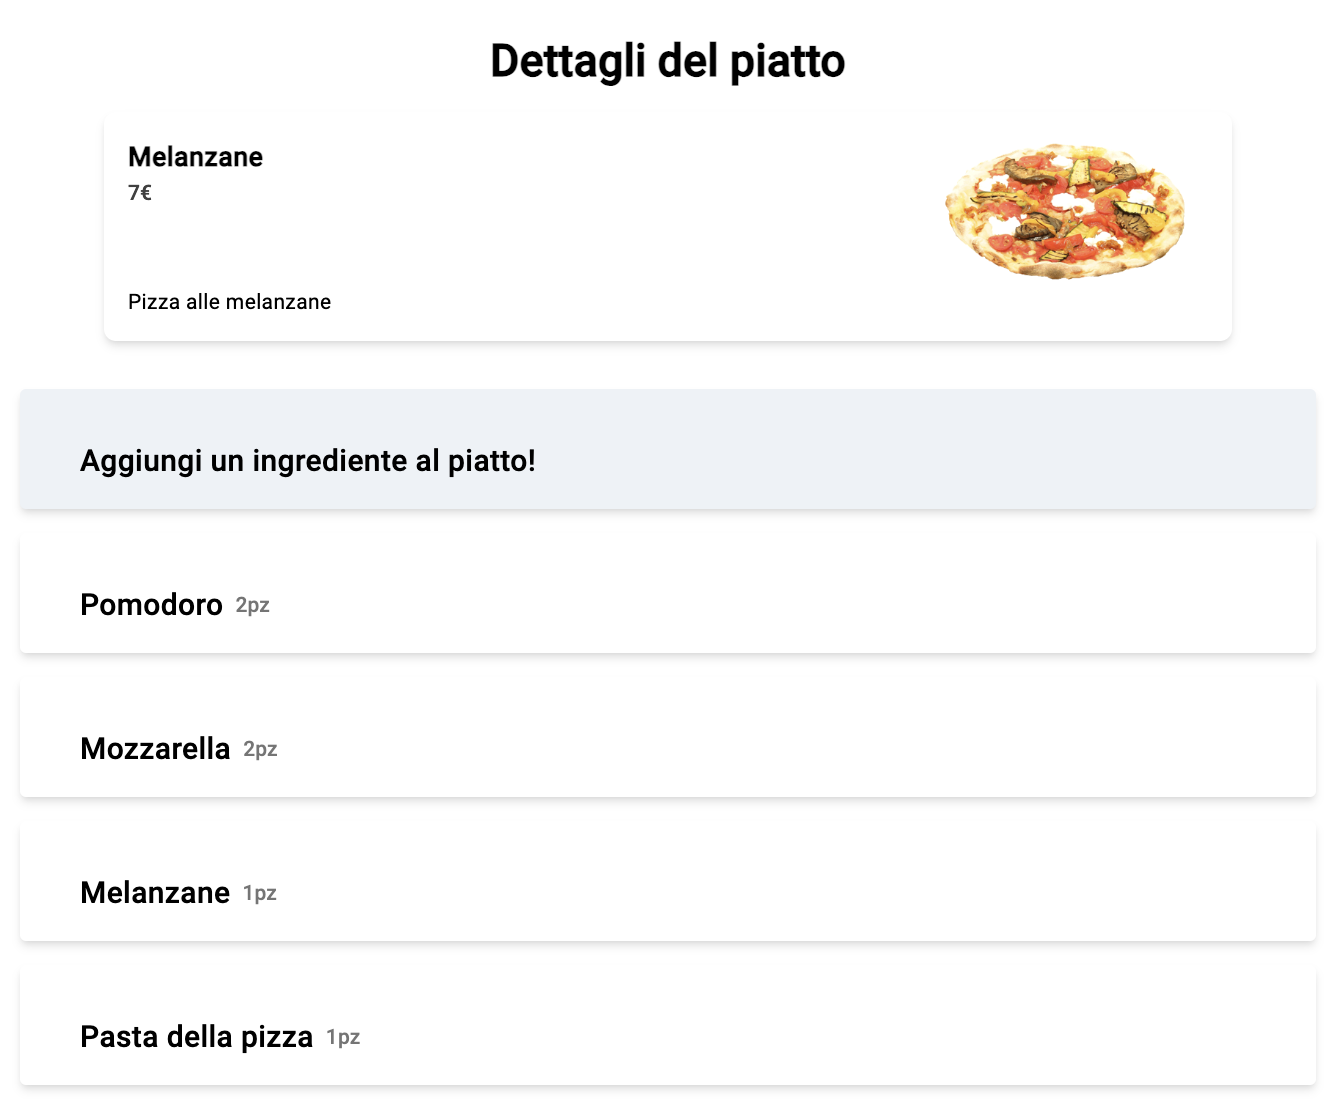
\includegraphics[width=0.8\textwidth]{PB/manuale-utente/dettaglio-piatto-ristoratore.png}
    \caption{Pagina di dettaglio di un piatto per il ristoratore}
\end{figure}

Si accede a questa pagina cliccando su un piatto nella lista dei piatti. Qui
puoi visualizzare i dettagli del piatto e i suoi ingredienti. In questa pagina
sono disponibili le seguenti funzionalità:
\begin{itemize}
	\item \textbf{Modifica piatto}: cliccando sul piatto, esso si trasforma in
		nel \textit{form} di creazione con i campi già compilati. Puoi modificare i
		campi e salvare le modifiche cliccando sul pulsante \texttt{Modifica
		piatto}. Se l'operazione va a buon fine, vieni reindirizzato alla
		pagina di visualizzazione dei piatti e viene visualizzato un messaggio
		di conferma di avvenuta modifica del piatto; altrimenti viene
		visualizzato un messaggio di errore;

	\item \textbf{Elimina piatto}: cliccando sul piatto, esso si trasforma nel
		\textit{form} di creazione con i campi già compilati. In fondo al \textit{form} è presente
		un bottone \texttt{Elimina piatto}. Cliccando su questo bottone, il
		piatto viene eliminato. Viene visualizzato un messaggio di conferma e
		vieni reindirizzato alla pagina di visualizzazione dei piatti; oppure 
		viene visualizzato un messaggio di errore dell'operazione;

	\item \textbf{Aggiungi ingrediente}: sotto ad un piatto è presente un
		pulsante \texttt{Aggiungi un ingrediente al piatto!}. Cliccando su
		questo pulsante si apre un \textit{form} che ti permette di aggiungere un
		ingrediente al piatto. Il \textit{form} richiede:
		\begin{itemize}
			\item Ingrediente: un ingrediente presente negli ingredienti del tuo
				ristorante. Cliccando su questo campo si apre un menu a
				tendina con tutti gli ingredienti presenti nel tuo ristorante;

			\item Quantità: la quantità dell'ingrediente da aggiungere al piatto.
		\end{itemize}

		Dopo aver compilato il \textit{form}, puoi salvare l'ingrediente cliccando sul
		pulsante \texttt{Aggiungi ingrediente}. Se l'operazione va a buon fine,
		viene visualizzato un messaggio di conferma di avvenuta aggiunta
		dell'ingrediente al piatto; altrimenti viene visualizzato un messaggio
		di errore;

	\item \textbf{Modifica di un ingregrediente del piatto}: sotto al pulsante
		di aggiunta di un ingrediente è presente un elenco degli ingredienti
		del piatto. Cliccando su un ingrediente si apre un \textit{form} che ti permette
		di modificare la quantità dell'ingrediente dal piatto. Dopo aver 
		modificato la quantità
		dell'ingrediente, puoi salvare le modifiche cliccando sul pulsante
		\texttt{Modifica ingrediente}. Se l'operazione va a buon fine, viene visualizzato un
		messaggio di conferma di avvenuta modifica dell'ingrediente; altrimenti
		viene visualizzato un messaggio di errore;

	\item \textbf{Elimina ingrediente}: sotto al pulsante di aggiunta di un
		ingrediente è presente un elenco degli ingredienti del piatto. Cliccando
		su un ingrediente si apre un \textit{form} che ti permette di modificare la
		quantità dell'ingrediente dal piatto. In fondo al \textit{form} è presente un
		bottone \texttt{Elimina ingrediente}. Cliccando su questo bottone,
		l'ingrediente viene eliminato dal piatto. Viene visualizzato un messaggio
		di conferma e viene visualizzato un messaggio di conferma di avvenuta
		eliminazione dell'ingrediente dal piatto; altrimenti viene visualizzato
		un messaggio di errore dell'operazione.
\end{itemize}

\subsection{Prenotazioni}

\begin{figure}[htbp]
    \centering
	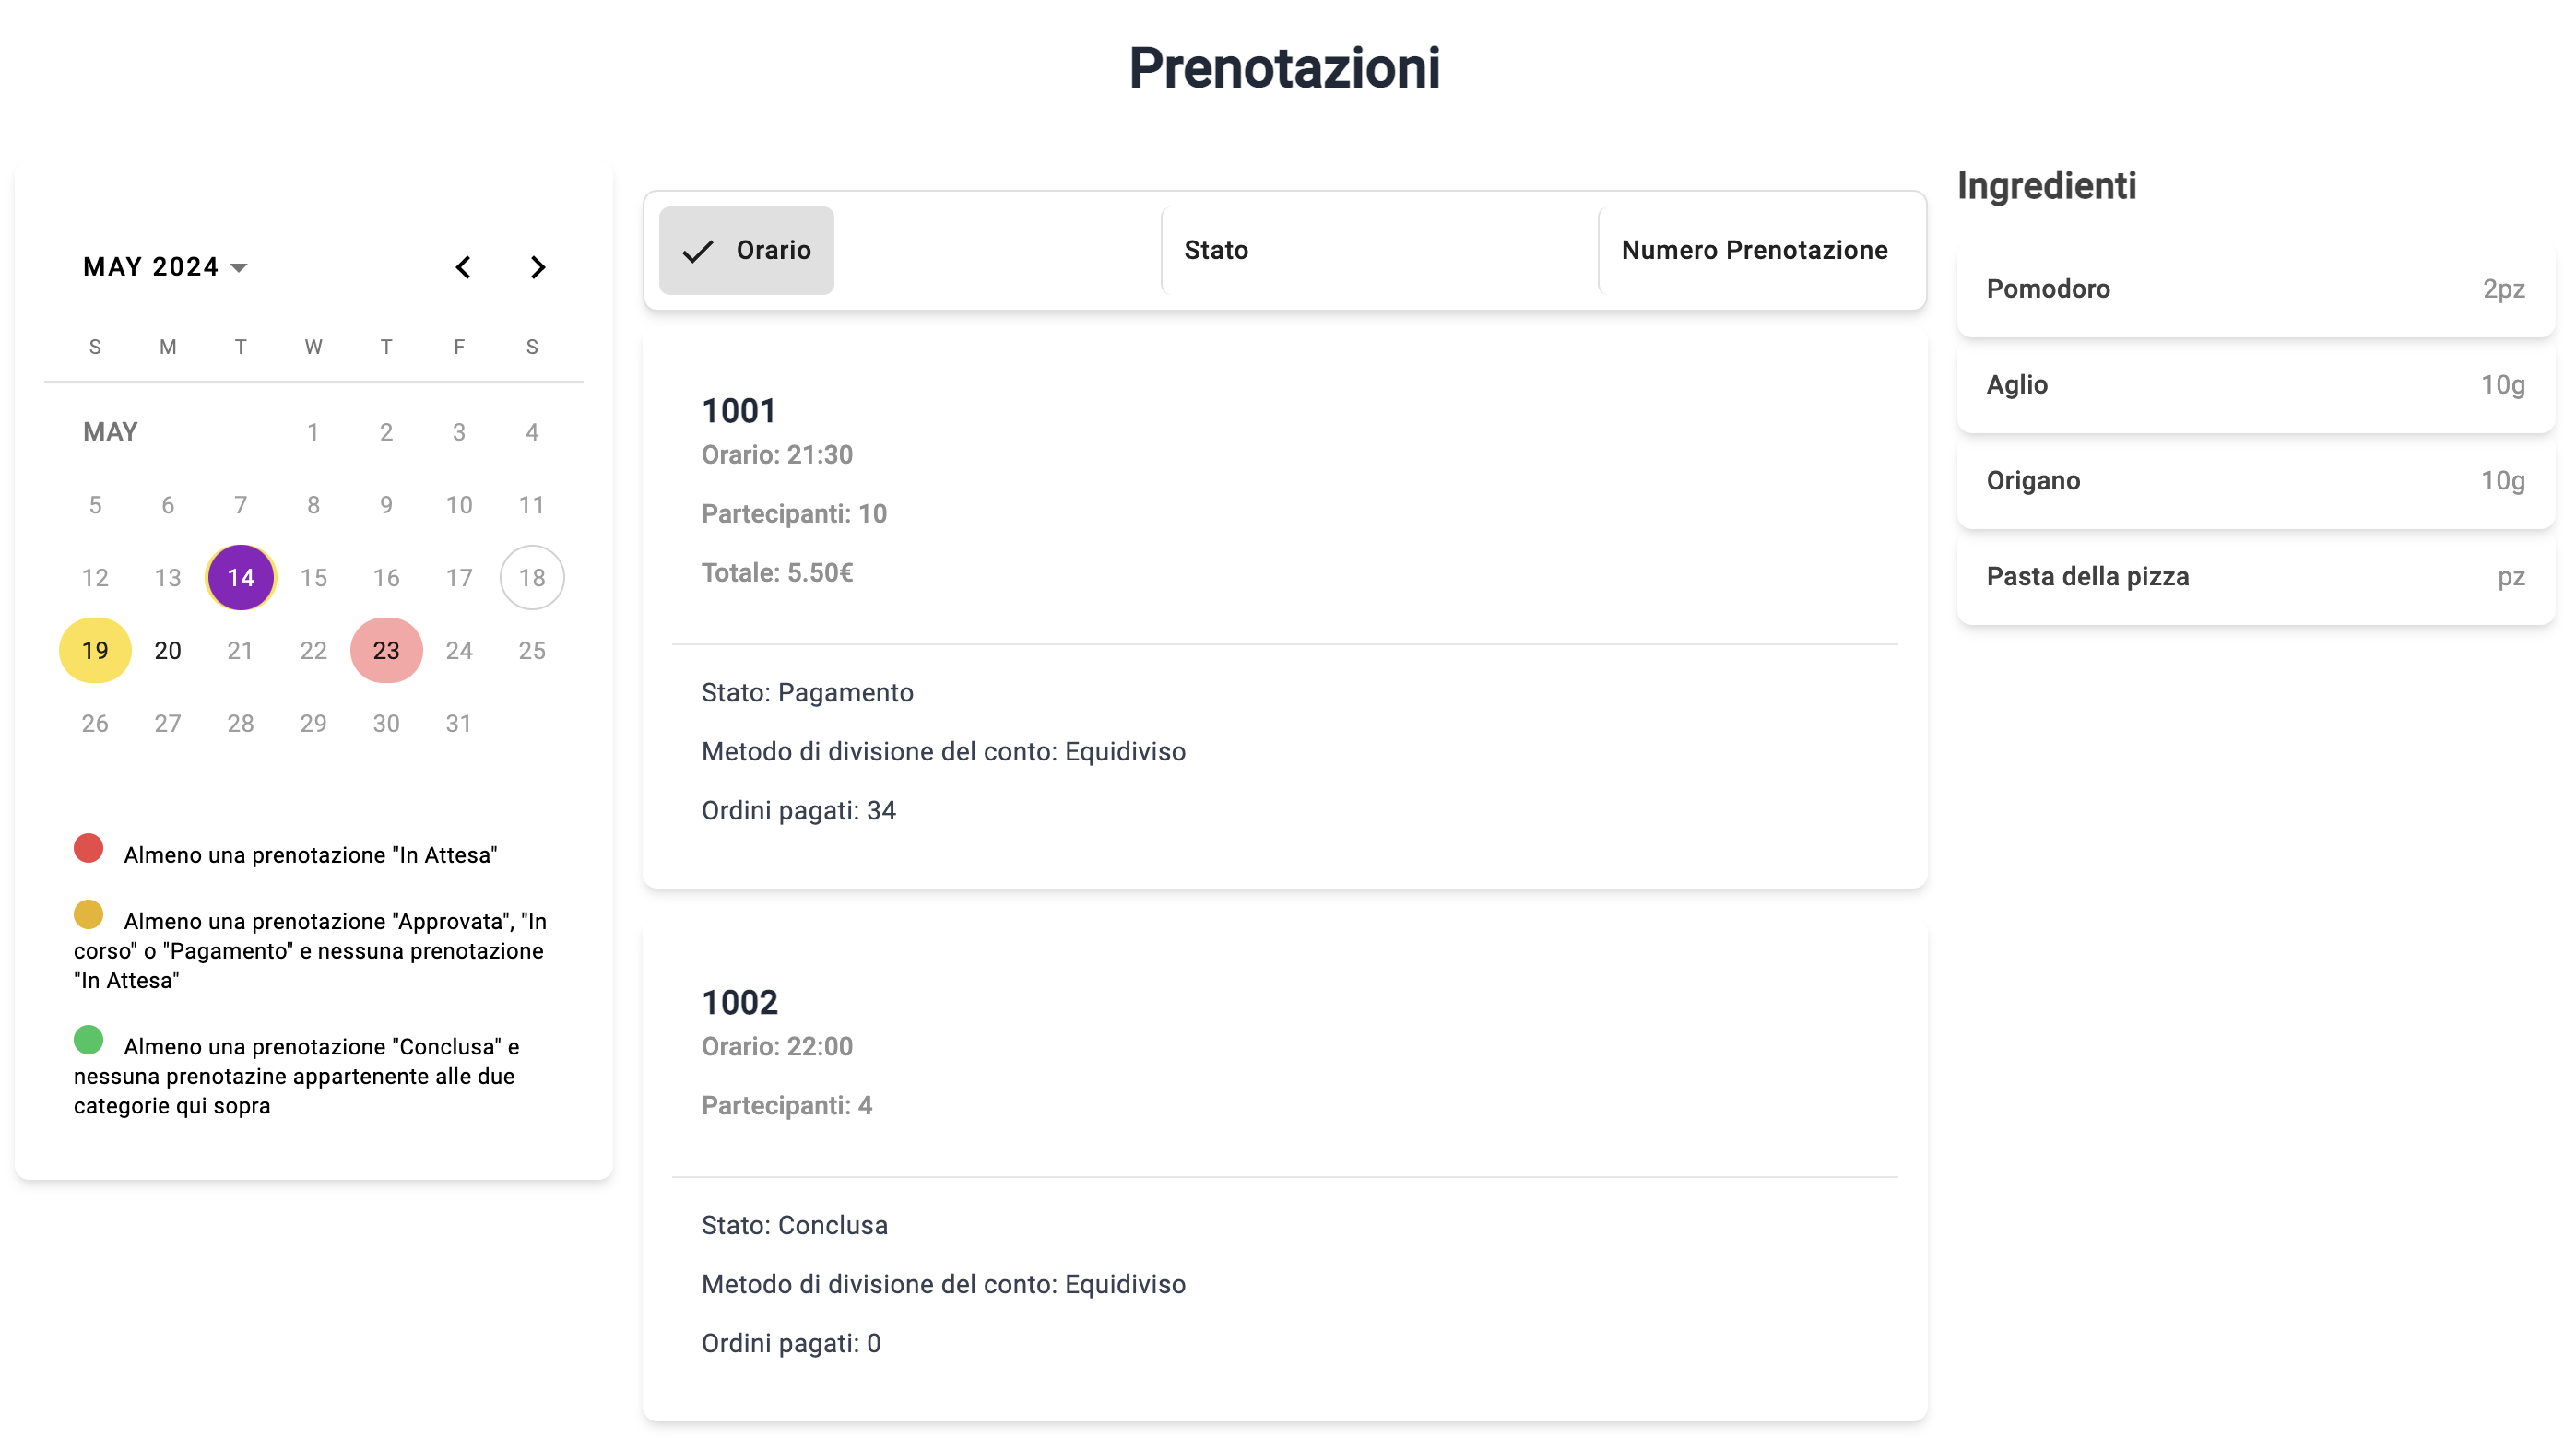
\includegraphics[width=0.8\textwidth]{PB/manuale-utente/prenotazioni-ristoratore.png}
	\caption{Pagina di visualizzazione delle prenotazioni per il ristoratore}
\end{figure}

Si accede a questa pagina cliccando su \texttt{Prenotazioni} nella barra di
navigazione. La pagina delle prenotazioni è divisa in tre sezioni:
\begin{itemize}
	\item \textbf{calendario}: questa sezione occupa la porzione sinistra della
		pagina. In questa sezione è possibile selezionare un giorno e
		visualizzare il colore dei giorni e i giorni cliccabili. Infatti, i
		quelli colorati di rosso indicano che c'è almeno una prenotazione nello
		stato "In attesa", ovvero c'è almeno una prenotazione, per la quale tu
		devi ancora confermare la disponibilità; i giorni colorati di giallo
		indicano che non ci sono prenotazioni "In attesa", ma c'è almeno una
		prenotazione in uno degli stati "Approvata", "In corso" oppure
		"Pagamento"; i giorni colorati di verde indicano che non ci sono
		prenotazioni appartenenti alle categorie precedenti, ma c'è almeno una
		prenotazione nello stato "Conclusa". I giorni cliccabili, ma non
		colorati hanno solo prenotazioni nello stato "Rifiutata" oppure
		"Annullata". Selezionando un giorno del calendario si aggiorna la lista
		delle prenotazioni in base al giorno selezionato;

	\item \textbf{lista delle prenotazioni}: questa è la centrale della pagina.
		In questa sezione sono elencate tutte le prenotazioni relative al giorno
		selezionato nel calendario. Cliccando su una prenotazione sei
		reindirizzato alla pagina di dettaglio della prenotazione. In cima alla
		lista delle prenotazioni sono presenti tre pulsanti per riordinare le
		prenotazioni rispettivamente: \texttt{Orario}, \texttt{Stato} e
		\texttt{Numero prenotazione}. Cliccando su uno di questi pulsanti si
		riordinano le prenotazioni in base al campo selezionato;

	\item \textbf{lista degli ingredienti}: questa sezione occupa la porzione
		destra della pagina. In questa sezione sono elencati tutti gli
		ingredienti necessari per soddisfare le prenotazioni del giorno
		selezionato. Si noti che le prenotazioni "Annullata" e "Rifiutata" non
		sono considerate, mentre le prenotazioni "In attesa" sono considerate.
\end{itemize}

\subsection{Dettaglio prenotazione}

\begin{figure}[htbp]
    \centering
	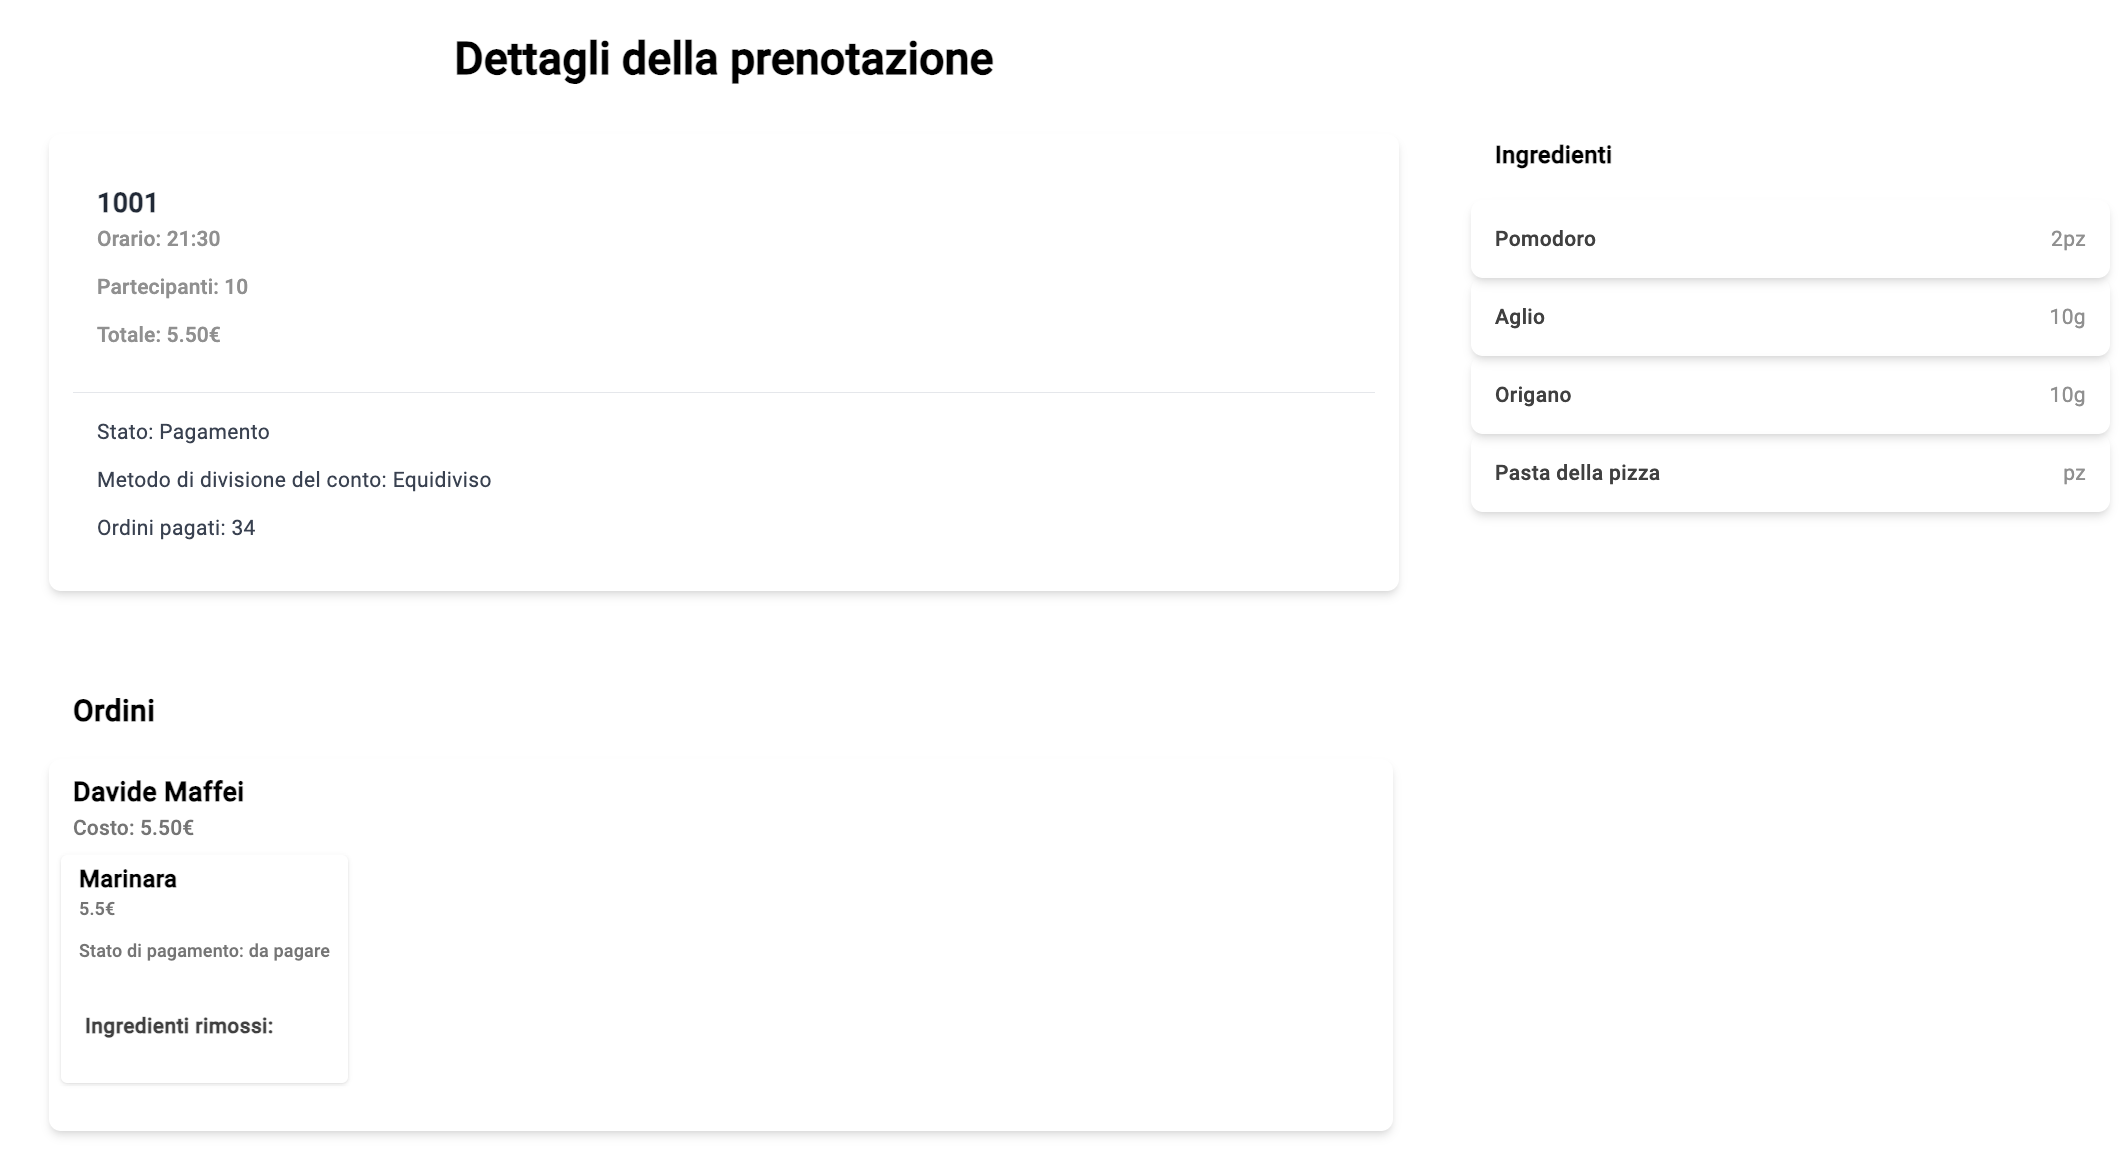
\includegraphics[width=0.8\textwidth]{PB/manuale-utente/dettaglio-prenotazione-ristoratore.png}
    \caption{Pagina di dettaglio di un'ordinazione per il ristoratore}
\end{figure}

Si accede a questa pagina cliccando su una prenotazione nella lista delle
prenotazioni. Qui puoi visualizzare i dettagli della prenotazione e i piatti
ordinati. Cliccando sui dettagli di una prenotazione si aprirà un \textit{form} che
permette di modificare lo stato della prenotazione. Dopo aver modificato lo
stato della prenotazione, puoi salvare le modifiche cliccando sul pulsante
\texttt{Salva}. Se l'operazione va a buon fine, vieni reindirizzato alla pagina
delle prenotazioni e viene visualizzato un messaggio di conferma di avvenuta
modifica della prenotazione; altrimenti viene visualizzato un messaggio di errore.
Sotto i dettagli della prenotazione sono elencati tutti i piatti ordinati divisi
per cliente. Infine, a destra della prenotazione e dei piatti ordinati, è
presente la lista degli ingredienti necessari per soddisfare la prenotazione.
